%=====================================================================
%  TokPress — full paper
%  Compile: pdflatex -> bibtex(optional) -> pdflatex x2
%=====================================================================
\documentclass[10pt,twocolumn]{article}

\usepackage[a4paper,margin=1.9cm]{geometry}
\usepackage{amsmath,amssymb,amsthm}
\usepackage{newtxtext,newtxmath}
\usepackage{booktabs}
\usepackage{microtype}
\usepackage{graphicx}
\usepackage{url}
\usepackage{algorithm}
\usepackage{algpseudocode}
\usepackage{tikz}
\usetikzlibrary{arrows.meta,positioning}
\usepackage[colorlinks=true,allcolors=blue]{hyperref}
\usepackage[capitalise,nameinlink]{cleveref}
\usepackage{titlesec}
\usepackage{caption}
\captionsetup{font=small,labelfont=bf}
\floatplacement{algorithm}{t}

\titleformat{\section}{\normalfont\large\bfseries}{\thesection}{0.6em}{}
\titleformat{\subsection}{\normalfont\normalsize\bfseries}{\thesubsection}{0.6em}{}

\theoremstyle{plain}
\newtheorem{theorem}{Theorem}[section]
\newtheorem{lemma}[theorem]{Lemma}
\newtheorem{proposition}[theorem]{Proposition}
\newtheorem{corollary}[theorem]{Corollary}
\theoremstyle{definition}
\newtheorem{definition}[theorem]{Definition}
\newtheorem{remark}[theorem]{Remark}
\newtheorem{fact}[theorem]{Fact}

\crefname{algorithm}{Algorithm}{Algorithms}
\Crefname{algorithm}{Algorithm}{Algorithms}

\newcommand{\B}{\mathcal{B}}
\newcommand{\V}{\mathcal{V}}
\newcommand{\KL}[2]{D\!\left(#1 \,\|\, #2\right)}
\newcommand{\FLAG}{\mathtt{FLAG}}

\begin{document}

\title{\vspace{-1.2cm}\textbf{TokPress: A Tokenizer-Domain Entropy Coder\\
with a Trained Dictionary and Order-1 Fallback Cascade}\\[0.4em]
\large Technical Report}

\author{Le Duc Minh\\[0.25em]
\small\texttt{minh.leduc.0210@gmail.com}}
\date{}
\maketitle

\begin{abstract}
\noindent
TokPress is a pure-Python lossless compressor that tokenizes input with the
released \texttt{o200k\_base} vocabulary, applies token-level LZ77, and
entropy-codes the result with rANS. All domain adaptation happens in a separate
object, \texttt{TokDict}, which supplies an LZ priming buffer,
a baked order-0 table, and order-1 tables for the most frequent previous-token
contexts, linked by a two-level escape chain so the model itself is never sent
with a record. On held-out structured logs (184 training / 46
test records), a trained \texttt{TokDict} brings the compressed/original ratio from
$0.808$ to $\mathbf{0.2565}$ --- below \texttt{gzip -9} ($0.728$) and
dictionary-free \texttt{zstd -19} ($0.737$), and within $1.29\times$ of
\texttt{zstd -19} with a matched trained dictionary ($0.195$). The gain is
schema-specific: a dictionary trained on the wrong kind of data buys nothing. In
bulk mode TokPress beats \texttt{gzip -9} on 4 of 6 corpora and \texttt{zstd -19}
outright on a short-prose corpus, including an exact tie with \texttt{zstd -19} on a
long-prose-novel prefix. Every reported ratio was verified by a byte-exact
round-trip check.
\end{abstract}

%---------------------------------------------------------------------
\section{Introduction}
%---------------------------------------------------------------------

General-purpose stream compressors like \texttt{gzip} and \texttt{zstd} learn their
model from the input. That cost is easy to amortize over a large file, but not over
the short, independent records that structured logs, telemetry events, and per-entity
metadata usually are.

Zstandard handles this setting with dictionary mode: a dictionary is trained offline
and shared with the decoder. We ask whether a subword tokenizer trained the same way
can do the equivalent job for small records. A token sequence turns multi-byte
dependencies into adjacent-token ones (\Cref{thm:mi}), so a static low-order token
model may capture structure that would need a higher-order byte model. We test this
with the full, unfiltered \texttt{o200k\_base} encoding (so byte fallback, and hence
\Cref{thm:invert}, always holds) and keep every trained component --- the LZ priming
buffer, the order-0 table, the order-1 context tables --- in an external
\texttt{TokDict} object rather than compiled into the codec.

The regime this targets is no longer a niche. Database engines now train per-collection
dictionaries over small, schema-homogeneous documents to cut storage and I/O cost, and
the IETF's RFC~9842 (Compression Dictionary Transport, 2025) standardized zstd/brotli
dictionary compression over HTTP, with "known-structure API responses" named as the
prime fit. A shared static model over many small records is where the industry is
already heading; this work is one concrete, open, end-to-end implementation of that
idea, with the tokenizer taking the role of the shared dictionary.

The short version of the results is that this works in the regime it targets and not
outside it. With a trained \texttt{TokDict}, small structured records compress
smaller than with any dictionary-free compressor we tried, and come within
$1.29\times$ of a matched-schema \texttt{zstd -19} dictionary
(\Cref{sec:target}) --- a much smaller gap than the $5$--$7\times$ a plain
per-record encoder starts from, though we do not close it. The gain is specific to
the training schema: in a cross-schema test (\Cref{sec:generalization}), a dictionary
trained on the wrong kind of record is no better than no dictionary at all. In
general-purpose bulk mode, a wider entropy-table precision, separate tables for match
metadata, an adaptive table that costs nothing to transmit, and a per-record
PPM-style order-1 coder let TokPress beat \texttt{gzip -9} on 4 of 6 whole-file
 corpora and \texttt{zstd -19} outright on short prose (\Cref{sec:bulk}).

TokPress is open source: the implementation, wire-format documentation, and the
benchmark harness are available at \url{https://github.com/LakoreAI/tokpress}.

\paragraph{Contributions.}
\begin{enumerate}\itemsep2pt
\item A rate equation that separates the codec's sources of redundancy, plus a
coding-identity/KL treatment of tokenization (\Cref{sec:theory}, \Cref{app:proofs}).
\item A codec over the full released tokenizer: escape symbols so entropy tables
never run out of alphabet, a 64-bit rANS state at $M=2^{16}$ with the overflow risk
checked, match metadata coded in its own tables, and a chunked-adaptive table that
costs nothing to transmit (\Cref{sec:system}).
\item \texttt{TokDict}, an external trained dictionary (priming buffer, baked order-0,
order-1 cascade), with an honest account of when it helps and when it does not,
including a cross-schema test on a genuinely different record type
(\Cref{sec:results,sec:generalization}).
\item Bulk-mode measurements on six corpora --- including a Wikipedia-XML dump and a
long prose novel --- against \texttt{gzip}/\texttt{bz2}/\texttt{lzma}/
\texttt{zstd}/\texttt{brotli}/\texttt{lz4} and a tokenize-then-byte-compress
baseline (\Cref{sec:bulk}).
\end{enumerate}

%---------------------------------------------------------------------
\section{Related Work}
%---------------------------------------------------------------------

\paragraph{Entropy coding.} TokPress uses the range variant of asymmetric numeral
systems \cite{duda2009}. We use a static table rather than an online model because of
the Krichevsky--Trofimov redundancy bound for sequentially estimated models
\cite{kt1981}; see \Cref{sec:bake}.

\paragraph{Dictionary and LZ compression.} The sliding-window LZ77 family
\cite{zl1978} is asymptotically optimal \cite{wynerziv1994}, but its finite-length
redundancy \cite{louchard1997} matters at the record sizes we care about
(\Cref{sec:crossover}). Zstandard \cite{rfc8478}, including its \verb|--train|
dictionary mode, is our main comparison point. FemtoZip \cite{femtozip}, which shares
a dictionary across small independent documents, motivated the dictionary-priming
scheme in \Cref{sec:dict}. Shared static dictionaries are now a production pattern:
RFC~9842 standardizes dictionary compression for HTTP, and document databases
(MongoDB, Amazon DocumentDB) train per-collection dictionaries over small JSON
documents. For streaming logs, LogLite \cite{loglite2025} achieves strong
compression without any pre-training by adapting to the log structure on the fly; our
batch mode (\Cref{sec:system}) is the static-dictionary counterpart of that idea for
archival, write-once workloads.

\paragraph{Subword tokenization.} The relevant methods are BPE \cite{gage1994,
sennrich2016}, SentencePiece \cite{kudo2018,kudo2018sp}, and byte-level BPE
\cite{radford2019}; see Mielke et al.\ \cite{mielke2021} for a survey of
open-vocabulary tokenization. A tokenizer's compression quality is not merely an
implementation detail: compression is a reliable intrinsic signal of tokenizer
quality that correlates with downstream model performance
\cite{goldman2024,zouhar2023}, and BPE is not always the best segmentation for
pretraining quality \cite{bostrom2020}. TokPress uses the released
\texttt{o200k\_base} piece set
\cite{tiktoken2024} unfiltered, and deliberately does not restrict it per domain
(\Cref{sec:system}): a restricted piece set is only a valid tokenizer if it forms a
complete hierarchical BPE merge chain, which mining a subset by longest-match over a
training corpus does not guarantee.

\paragraph{Modeling as compression.} Del\'{e}tang et al.\ \cite{deletang2023} treat
sequence modeling and compression as the same problem, and neural models are used
directly as text compressors --- DeepZip \cite{deepzip2018} pairs a recurrent
predictor with an arithmetic coder, LLMZip \cite{llmzip2023} uses an LLM's
next-token probabilities, and compression efficiency has been shown to
track model capability almost linearly \cite{huang2024compression}. We work with a
static, non-neural model meant for short records at moderate computational cost.

\paragraph{Vocabulary sizing.} Heaps' \cite{heaps1978} and Zipf's \cite{zipf1949}
laws underlie the rate--fertility trade-off of \Cref{sec:vocab}; Llama~3
\cite{llama3} and \texttt{o200k\_base} \cite{tiktoken2024} are useful real-world
vocabulary-size reference points.

%---------------------------------------------------------------------
\section{System Description}\label{sec:system}
%---------------------------------------------------------------------

The encoder tokenizes the input, applies LZ77 to the token sequence, and then
entropy-codes the result. One tokenizer is used for everything; where domain
adaptation happens is described below. \Cref{fig:pipeline} shows the TokPress
pipeline; the formal encode and decode procedures are given in
\Cref{alg:encode,alg:decode}.

\begin{figure*}[t]
\centering
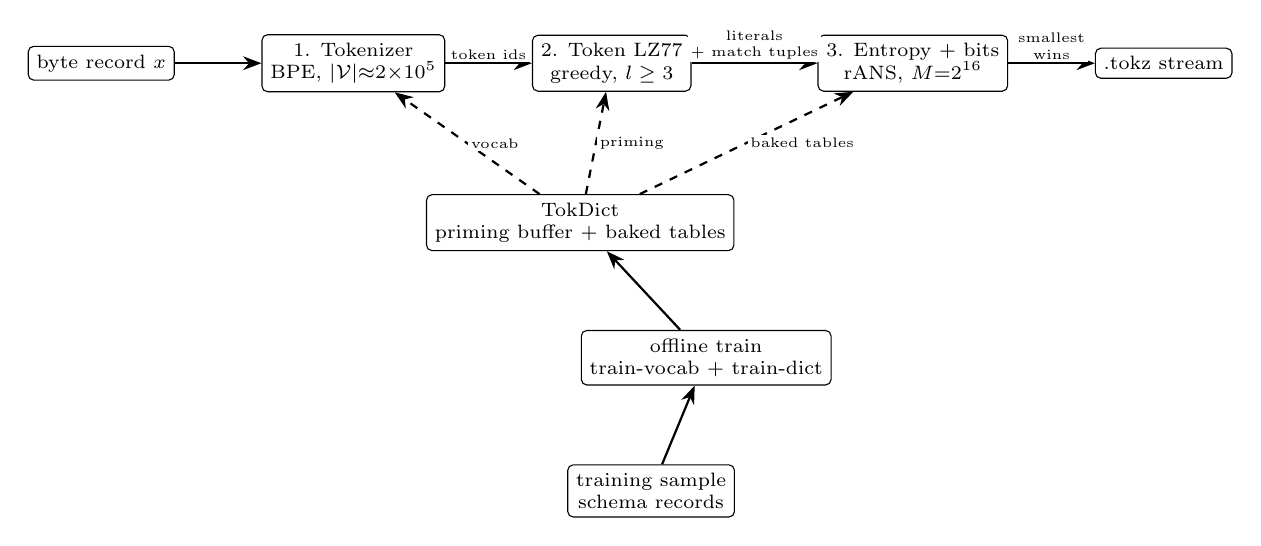
\begin{tikzpicture}[
  box/.style={draw, rounded corners=2pt, align=center, inner sep=3pt, font=\scriptsize},
  arr/.style={-{Stealth}, thick},
  darr/.style={-{Stealth}, thick, dashed},
  lbl/.style={font=\tiny, fill=white, inner sep=1pt, align=center},
]
  \node[box] (in) {byte record $x$};
  \node[box, right=11mm of in] (tok) {1. Tokenizer\\ BPE, $|\V|{\approx}2{\times}10^5$};
  \node[box, right=11mm of tok] (lz) {2. Token LZ77\\ greedy, $l \ge 3$};
  \node[box, right=16mm of lz] (ent) {3. Entropy + bits\\ rANS, $M {=} 2^{16}$};
  \node[box, right=11mm of ent] (out) {.tokz stream};

  \draw[arr] (in) -- (tok);
  \draw[arr] (tok) -- node[lbl,above]{token ids} (lz);
  \draw[arr] (lz) -- node[lbl,above]{literals\\+ match tuples} (ent);
  \draw[arr] (ent) -- node[lbl,above]{smallest\\ wins} (out);

  \node[box, below=13mm of lz, xshift=-4mm] (dict) {TokDict\\ priming buffer + baked tables};
  \node[box, below=10mm of dict, xshift=16mm] (train) {offline train\\ train-vocab + train-dict};
  \node[box, below=10mm of train, xshift=-7mm] (sample) {training sample\\ schema records};

  \draw[darr] (dict) -- node[lbl,right]{vocab} (tok);
  \draw[darr] (dict) -- node[lbl,right]{priming} (lz);
  \draw[darr] (dict) -- node[lbl,right]{baked tables} (ent);
  \draw[arr] (train) -- (dict);
  \draw[arr] (sample) -- (train);
\end{tikzpicture}
\caption{The TokPress pipeline: tokenize $\to$ token-level LZ77 $\to$ entropy-coded
bitstream, with the trained \texttt{TokDict} supplying the vocabulary, an LZ priming
buffer (so matches can reach into other records), and baked order-0/order-1 tables.}
\label{fig:pipeline}
\end{figure*}

\paragraph{1. Tokenizer.} The vocabulary $\V$ is the full, unfiltered, released
\texttt{o200k\_base} encoding ($|\V| \approx 2\times10^5$), used exactly as
published via its byte-exact \texttt{\_encode\_bytes}/\texttt{decode\_bytes} pair, so
arbitrary binary input (not only valid UTF-8) round-trips exactly. Byte-level
fallback ($\B \subseteq \V$) is guaranteed by \texttt{o200k\_base} itself, so
\Cref{thm:invert} applies unconditionally. We never restrict the vocabulary by
domain, because a restricted vocabulary is only valid if it forms a complete BPE
merge chain, and mining pieces by longest-match does not guarantee that. A domain
vocabulary trained by the project's \texttt{train-vocab}
tool can be substituted; the codec is tokenizer-agnostic.

\paragraph{2. Token-level LZ77.} A greedy hash-based parser works on token IDs.
History is optionally primed with a \emph{priming buffer} from a trained
\texttt{TokDict} (\Cref{par:tokdict}; up to 8192 tokens by default, a trainable
parameter), so matches can refer to material learned from other records. Without a
\texttt{TokDict}, history is empty and every record is compressed on its own. A match
of length $l$ costs four tokens, so matches are emitted only when $l \ge 3$
(\Cref{rem:threshold}). The match-flag symbol is the tokenizer's own vocabulary size,
so it never collides with a real token id.

\paragraph{3. Entropy coding.} A scalar rANS coder runs at precision
$M = 2^{16} = 65536$ (table-log 16; \Cref{sec:instantiation} explains why this needs
a 64-bit coder state). The encoder builds whichever of eight modes apply and keeps
the smallest (\Cref{alg:encode}):
\begin{itemize}\itemsep1pt
\item \textbf{raw}: fixed-width bit-packed tokens, the universal fallback when
nothing else applies or wins;
\item \textbf{sparse order-0}: a per-record table over the record's own distinct
symbols, with a reserved \emph{escape symbol} for anything beyond the $M-1$ most
frequent --- without this, a record with more than $M$ distinct symbols (ordinary
prose can, at a small $M$) would have no valid table and would silently fall back to
raw bit-packing;
\item \textbf{split}: LZ match metadata (the distance-high, distance-low, and length
bytes of a match tuple) is coded in its own three small tables, plus a role-bit table
distinguishing literals from match positions, all separate from the literal-token
table. Match-metadata bytes are near-uniform over $[0,255]$, a completely different
distribution from the literal tokens' Zipfian one; mixing them in one table dilutes
both. Measured directly, separation saves $6$--$16\%$ of the entropy-coded payload;
\item \textbf{chunked adaptive order-0}: no table is transmitted at all. Each chunk
after the first is coded against a Laplace-smoothed count of the chunks that came
before it, so the decoder derives the identical table from what it has already
decoded (\Cref{sec:bake} explains why we did not attempt fully per-symbol adaptive
coding);
\item \textbf{adaptive split}: the previous two combined --- match metadata stays in
static small tables while the literal sub-stream gets the chunked-adaptive treatment.
The two savings are largely independent, so a record can win from either or both;
\item \textbf{\texttt{TokDict} order-0/order-1 cascade} (\Cref{par:tokdict}): the
only mode with pre-trained, cross-record state, used only when a \texttt{TokDict} is
supplied;
\item \textbf{per-record PPM order-1}: an adaptive order-1 cascade over the whole
token stream --- the previous token's context table is tried first, an escape from
it falls through to a Laplace-smoothed order-0 table that always covers the symbol,
and each context reserves a count-based (PPMC-style) escape share, so a low-support
context mostly falls through and never hurts;
\item \textbf{PPM split}: the same order-1 cascade applied to the literal
sub-stream, with match metadata in its own tables (the two wins stack).
\end{itemize}
(An empty-input fallback handles the zero-byte edge case.)

\begin{algorithm}[t]
\caption{TokPress encode}
\label{alg:encode}
\begin{algorithmic}[1]
\Require input bytes $x$; optional \texttt{TokDict} $\Theta$
\Ensure a single-record TokPress stream
\State $t \gets \Call{Tokenize}{x}$ \Comment{byte-exact, arbitrary binary}
\State $s \gets \Call{LZ77}{t}$ \Comment{greedy; primed with $\Theta$'s buffer if given}
\State $C \gets \{\Call{Raw}{s}, \Call{Sparse}{s}, \Call{Split}{s}\}$
\State $C \gets C \cup \{\Call{Adaptive}{s}, \Call{AdaptiveSplit}{s}\}$
\If{a dictionary $\Theta$ is given}
    \State add $\Call{DictCascade}{s, \Theta}$ to $C$ \Comment{see \Cref{alg:tokdict-cascade}}
\EndIf
\State \Return $\arg\min_{c \in C} |c|$ \Comment{every candidate is built; the smallest wins}
\end{algorithmic}
\end{algorithm}

\begin{algorithm}[t]
\caption{TokPress decode}
\label{alg:decode}
\begin{algorithmic}[1]
\Require a TokPress stream; optional \texttt{TokDict} $\Theta$
\Ensure the original bytes $x$
\State parse the magic, version, mode, and payload header
\State decode the LZ-token stream with the mode's rANS tables \Comment{escape lists resolved in order}
\State $t \gets \Call{LZDecompress}{s, \Theta.priming}$
\State \Return $\Call{Detokenize}{t}$
\end{algorithmic}
\end{algorithm}

\paragraph{\texttt{TokDict}: an external, explicitly-trained dictionary.}
\label{par:tokdict}
All trained, domain-adapted state lives in an external, opt-in object, trained by the
caller on a sample of representative records (\Cref{alg:tokdict-train}), saved to a
portable file, and supplied explicitly at compress/decompress time. Training
accumulates: (i) a priming buffer (the sample records' own token streams,
concatenated up to a cap); (ii) order-0 counts over the resulting LZ-token stream;
and (iii) order-1 counts for every (previous-token, next-token) pair observed. The
order-0 and every order-1 table use the same escape-capping construction as the
sparse mode, but not the same escape share: order-0 reserves a small fixed $1.5\%$,
while each context table reserves a PPMC-style count-based share estimated from its
own counts, because a context table sees far
fewer observations than order-0 does, so ``this specific transition was not in
training'' is common for it, not rare (\Cref{sec:order1} has the ablation). Only the
top 64 contexts with at least 20 observed transitions get their own table; a
low-support context is simply never given one, at no cost. To encode a symbol whose
previous symbol has a trained context table, we try that table first; an escape
falls through to the order-0 table; an escape from \emph{that} carries the symbol's
value out-of-band as an explicit integer (\Cref{alg:tokdict-cascade}). Which table to
try depends only on the \emph{previous} symbol and the dictionary's fixed metadata
--- never on the current symbol's value --- so the decoder can derive the same
cascade from what it has already decoded, without transmitting anything about the
table choice.

\begin{algorithm}[t]
\caption{\texttt{TokDict} training}
\label{alg:tokdict-train}
\begin{algorithmic}[1]
\Require sample records $\{r_1, \dots, r_n\}$; tokenizer; cap $P$ on priming tokens
\Ensure a \texttt{TokDict} $\Theta = (\text{priming}, \text{order0}, \text{contexts})$
\State $t_i \gets \Call{Tokenize}{r_i}$ for each $i$
\State $\text{priming} \gets$ concatenation of the $t_i$, capped at $P$
\State $s_i \gets \Call{LZ77}{t_i}$ for each $i$
\State accumulate order-0 counts over all $s_i$; and order-1 counts for every adjacent pair
\State bake the order-0 table, capped to $M{-}1$ symbols plus one escape (share $1.5\%$)
\State keep the top-64 contexts with $\ge 20$ transitions; bake each with a PPMC-adaptive escape share
\State compute the 8-byte fingerprint; \Return $\Theta$
\end{algorithmic}
\end{algorithm}

\begin{algorithm}[t]
\caption{\texttt{TokDict} order-1 $\to$ order-0 $\to$ escape cascade (encode one symbol)}
\label{alg:tokdict-cascade}
\begin{algorithmic}[1]
\Require symbol $y$; previous symbol $x$; \texttt{TokDict} $\Theta$
\State $ctx \gets$ the trained context table for $x$, if one exists
\If{$y$ is in $ctx$}
    \State rANS-encode $y$ against $ctx$ \Comment{no fallback needed}
\ElsIf{$y$ is in the order-0 table}
    \State rANS-encode $y$ against the order-0 table; then a $ctx$-escape if $ctx$ exists
\Else
    \State append $y$ to the out-of-band escape list
    \State rANS-encode the order-0 escape; then a $ctx$-escape if $ctx$ exists
\EndIf
\State \Comment{encode calls are issued in reverse logical order --- see \Cref{sec:system}}
\end{algorithmic}
\end{algorithm}

\paragraph{Correctness.} The cascades were easy to get wrong, and three real bugs
were found and fixed only by testing many varied payloads rather than one fixed one.
First, rANS encodes in reverse logical order (\Cref{sec:bake}), so a position needing
a two-event cascade (e.g.\ context-then-order-0 fallback) must have its \emph{encode
calls} issued in the \emph{opposite} micro-order from how the decoder consumes them;
getting this backwards corrupts output only on inputs that exercise the escape path.
Second, in adaptive-split mode the escape list is built in a forward pass \emph{first}
(unlike every other mode, where it is built during the reverse loop), so reversing it
a second time at the end silently reordered escaped values --- again, only when a
record had more than one order-0 escape. Third, a table with exactly one active symbol
has frequency exactly $M$ (certainty), which needs $\log_2 M + 1$ bits, one more than
the field width used for every other frequency; transmitting it directly truncated
$2^{16}$ to $0$ on the wire. Transmitting frequency $-1$ instead (range
$[0, M{-}1]$) fixes this uniformly. All three were caught by tests that loop over many
payload shapes, random synthetic symbol streams, or extreme record sizes.

%---------------------------------------------------------------------
\section{Theoretical Foundation}\label{sec:theory}
%---------------------------------------------------------------------

Let $\B = \{0,\dots,255\}$ be the byte alphabet; a message is $x \in \B^*$ with
$|x| = n$. We write $H$ for entropy, $I$ for mutual information, and
$\KL{p}{q} = \sum_x p(x)\log_2 (p(x)/q(x))$ for KL divergence.

The coding identity --- the expected length under a mismatched model is the source
entropy plus a KL-divergence penalty, $\mathbb{E}_p[-\log_2 q(X)] = H(p)+\KL{p}{q}$ ---
is stated and proved in \Cref{app:proofs} (\Cref{lem:coding}); we use it throughout.
All formal statements below are collected in \Cref{app:proofs} and only the claims
are quoted here.

\subsection{Entropy invariance under tokenization}

\begin{definition}[Greedy longest-match tokenizer]
Fix $\V$ with $\B \subseteq \V$. The map $T:\B^* \to \V^*$ emits, at each position,
the longest piece of $\V$ that prefixes the remaining suffix, and advances by its
length. The concatenation map $\kappa: \V^* \to \B^*$ recovers the bytes.
\end{definition}

Tokenization is invertible and preserves source entropy (\Cref{thm:invert}): byte
fallback guarantees the greedy matcher never stalls, so $\kappa(T(x))=x$, $T$ is
injective, and $H(T(X)) = H(X)$. A direct consequence is that tokenization cannot
reduce the information content of a message --- every compression gain must come from
\emph{modeling}, never from the transform (\Cref{cor:nofreelunch}).

The bulk-mode results in \Cref{sec:bulk} are consistent with this: without a
domain-trained model, TokPress is a general LZ and entropy-coding pipeline and gets no
advantage from tokenization alone.

\subsection{Gain from token context}

Let $\bar\ell = |x|/m$ be the mean bytes per token, and $R_0^T = H(T_1)/\bar\ell$,
$R_1^T = H(T_1 \mid T_0)/\bar\ell$ the per-byte rates of order-0 and order-1 token
models. The per-byte difference between the two is the adjacent-token mutual
information, $R_0^T - R_1^T = I(T_0;T_1)/\bar\ell \ge 0$ (\Cref{thm:mi}).

Because a token spans an average of $\bar\ell$ bytes, the previous token carries
several bytes of context. For sources with multi-byte dependence, a first-order token
model may therefore hold more useful context than a first-order byte model. How big
the effect is depends on the source and tokenizer; \Cref{sec:order1} measures it on
held-out data via $I(T_0;T_1)$.

\begin{remark}[State-space reduction]\label{rem:states}
A byte-level order-$m$ model needs $256^m = 2^{8m}$ conditioning contexts; a
token-level order-1 model needs $K = |\V|$. At comparable context reach the ratio is
$2^{8\bar\ell}/K$, i.e.\ $2^{32}/2^{16} = 2^{16}$ at $\bar\ell = 4$, $K = 2^{16}$.
This is a statement about parameter count, not expressivity: token boundaries vary
with the input, and correlations inside a token are represented by the vocabulary
rather than by the context model.
\end{remark}

\subsection{Vocabulary sizing}\label{sec:vocab}

Let $K = |\V|$ and let $r(K) = a + \beta \ln K$ be the mean fertility
(Heaps-type growth, with $a \ge 1$ forced by byte fallback), and suppose token
ranks follow a Zipf law with exponent $\alpha$. Under that Zipf law the vocabulary
entropy grows like $\tfrac12\log_2 K$ at $\alpha=1$ (\Cref{lem:zipf}), and the
per-byte rate is monotone in $\log K$, so there is no interior optimum --- only a
knee (\Cref{prop:knee}).

For $\alpha \approx 1$, $H(K)\approx\tfrac12\log_2 K+c$. Tokenizers with
$K\approx50$--$128$k commonly yield $9.5$--$10.5$ bits/token, which matches
$O(\tfrac12\log_2 K)$ growth; a $\log_2(\ln K)$ model would predict only about $3.5$
bits at $K=2^{16}$.

The useful operating point is a knee, not an interior minimum. Once the corpus's
useful subword inventory is covered, extra entries add little fertility while table
cost keeps growing with $K$. That argues for capping the \emph{tokenizer}'s vocabulary
at a domain-appropriate $K$; TokPress instead uses the full released
\texttt{o200k\_base} vocabulary (\Cref{sec:system}) and applies the cap at the
\emph{entropy-table} layer instead --- $M{-}1$ symbols per baked table with an escape
for the rest (\Cref{sec:instantiation}) --- since a real, valid tokenizer vocabulary
cannot be truncated post hoc. We did not fit $a$, $\beta$, or $\alpha$ to locate the
knee for $\V$'s real $K\approx2\times10^5$ (\Cref{sec:limits}).

\subsection{Token-level LZ77 and the small-record crossover}\label{sec:crossover}

\begin{definition}[Match and greedy parse]
A match at position $i$ with distance $d \le D$ and length $l \le L$ requires
$t_{i+k} = t_{i-d+k}$ for $k < l$. The parser replaces $l$ tokens by the 4-token
tuple $(\FLAG,\ \lfloor d/2^8\rfloor,\ d \bmod 2^8,\ l)$, with
$\FLAG = |\V|$, escaping a literal $\FLAG$ as $(\FLAG,0,0,0)$. The implementation
uses $D = 2^{15}$, $L = 255$.
\end{definition}

\begin{remark}[Match-length threshold]\label{rem:threshold}
A match of length $l$ costs 4 \emph{tokens}, so raw \emph{token count} only decreases
for $l \ge 5$. But we minimize entropy-coded \emph{bits}, not token count, and once
match metadata is coded separately in cheap, concentrated tables
(\Cref{sec:system}), a match's 4-token overhead can cost far fewer bits than the
$l{-}1$ literal tokens it replaces, even at $l=3$. Measured on every corpus we tried,
$l\ge3$ compressed $3$--$7\%$ smaller than $l\ge5$ under the current architecture;
under a plain fixed-width bit-packed or single-shared-table encoding the reverse held
(\Cref{sec:dict}), which is why an earlier revision moved the threshold up to 5 and
this one moved it back down.
\end{remark}

Sliding-window LZ77's rate carries a finite-length redundancy of
$\Theta(\log\log N/\log N)$ bits/byte over $N$ bytes (\Cref{thm:lzrate}).
Representative asymptotic estimates are roughly $0.3$--$0.5$ bits/byte at
$N=200$\,B, $0.1$ bits/byte at $N=1$\,MB, and $0.05$ bits/byte at $N=1$\,GB. The
finite-length term is therefore relevant for the short records we target.

\begin{remark}[The crossover]\label{rem:crossover}
A pretrained static model has no within-record learning term, so its rate is roughly
independent of $N$. A crossover $N^\star$ is expected where
\[
\frac{\hat H}{r} + \varepsilon_{\mathrm{coder}} + \frac{R_{\mathrm{header}}}{N}
\;<\; h + c\,\frac{\log\log N}{\log N},
\]
Our experiments cover records of about $200$--$540$\,B and bulk-file inputs. A size
sweep over per-record compression (\Cref{sec:sweep}) locates $N^\star$ for one
schema-homogeneous record family at roughly 1--2\,KB, where per-record adaptive
\texttt{zstd} overtakes the trained static model.
\end{remark}

\subsection{rANS and the master equation}

\begin{definition}[rANS step]
With frequencies $f_i > 0$, total $M = \sum_i f_i$, cumulative $c_i$, and
$q_i = f_i/M$: encoding symbol $i$ from state $s$ gives
$s' = \lfloor s/f_i \rfloor M + (s \bmod f_i) + c_i$; decoding sets
$b = s' \bmod M$, recovers the unique $i$ with $c_i \le b < c_i + f_i$, and returns
$s = f_i\lfloor s'/M\rfloor + (b - c_i)$. States are renormalized into
$[L, 2^{16}L)$ with $L = 16M$ (this ratio, not the absolute value of $L$, is what the
implementation holds fixed as $M$ changes --- \Cref{sec:instantiation}), emitting or
consuming 16-bit words.
\end{definition}

The rANS step is a bijection and decodes uniquely given the exact frequency model
(\Cref{thm:rans-correct}), and its expected per-symbol length under a mismatched
model $q$ against the true $p$ is $\sum_i p_i \log_2(M/f_i) = H(p)+\KL{p}{q}$
(\Cref{thm:rans-opt}). So model changes show up directly in the rate: vocabulary
selection and conditional modeling affect the mismatch term, while finite precision
adds a coder overhead.

\begin{remark}[Block flush cost]\label{rem:flush}
An interleaved coder flushing $W$ states of 32 bits per block of $M_b$ tokens pays
$\varepsilon_{\mathrm{flush}} = 32W/M_b$ bits/token. At $W = 8$, $M_b = 50$ (a single
log line) this is $5.12$ bits/token --- larger than the entire model term. For short
blocks the cost falls if fewer lanes are used or several records are coded in one
block so that $M_b \gg 32W$.
\end{remark}

The master rate equation, which separates the codec's redundancy sources, is stated
and proved in \Cref{app:proofs} (\Cref{thm:master}); its terms map to design choices
in \Cref{tab:ledger}.

\begin{table}[t]
\centering\small
\caption{Relation between codec design choices and the terms in
\Cref{thm:master}.}
\label{tab:ledger}
\begin{tabular}{@{}p{3.0cm}p{1.5cm}p{2.7cm}@{}}
\toprule
\textbf{Lever} & \textbf{Term} & \textbf{Mechanism} \\
\midrule
Trained \texttt{TokDict} & $\KL{\tilde p}{\tilde q}$ & concentrates long-range
dependence into adjacent-token MI \\
Order-1 modeling & $H(\tilde p)$ & recovers $I(T_0;T_1)/\bar\ell$ \\
Larger $M$ & $\varepsilon_{\mathrm{quant}}$ & finer frequency grid \\
Baked (shared) model & $\varepsilon_{\mathrm{header}}$ & no per-record table on
the wire \\
Static, no adaptation & $R_{\mathrm{model}}$ & removes KT learning cost \\
Few lanes / batching & $\varepsilon_{\mathrm{flush}}$ & fewer flushed states \\
Threshold $l \ge 3$ & $\varepsilon_{\mathrm{LZ}}$ & no expand-by-one matches \\
\bottomrule
\end{tabular}
\end{table}

By \Cref{thm:invert}, tokenization does not change the source entropy. Its role is to
change how much model mismatch is attainable at a fixed context order.

\subsection{Static versus adaptive models}\label{sec:bake}

An online-adaptive frequency model pays a Krichevsky--Trofimov redundancy
\cite{kt1981} of roughly
\[
R_{\mathrm{model}} \approx \frac{C(K-1)}{2}\log_2 \frac{M}{C}\ \text{bits}
\]
over $C$ context classes, $K$ symbols, and $M$ tokens. At $C=256$ and $K=2^{16}$,
that is about $8.4\times10^6$ parameters, and the redundancy drops below
$\varepsilon$ bits/token only when $M/\log_2(M/C)\gg10^8$ --- far beyond the roughly
50 tokens in a 200\,B record. So TokPress bakes its \texttt{TokDict} tables statically
rather than adapting them per-symbol online: training cost is shared across the
corpus, and model error shows up in the fixed $\KL{p}{q}$ term instead of an online
learning cost. \Cref{tab:progression} shows the measured progression from no
dictionary to a fully trained order-0/order-1 \texttt{TokDict}. Inside a single
record with no shared training data, the same argument runs the other way:
\Cref{sec:order1} reports that a per-record static order-1 table, with no corpus to
amortize its transmission cost, consistently loses to plain order-0 --- the opposite
of the corpus-amortized case, and the reason \texttt{TokDict}'s order-1 tables are
trained once across many records rather than fit fresh per record. The chunked-adaptive
mode (\Cref{sec:system}) is a smaller, safer step in the online direction: it never
transmits a table, only adapts an order-0 model, and only within records long enough
to have several chunks of history.

Formally, over $N_{\mathrm{tot}}$ corpus bytes and per-record token count
$M_{\mathrm{rec}}$,
\[
b = \frac{\hat H}{r} + \varepsilon_{\mathrm{quant}}
+ \varepsilon_{\mathrm{flush}}
+ \frac{R_{\mathrm{vocab}} + R_{\mathrm{tables}}}{N_{\mathrm{tot}}}
+ \frac{R_{\mathrm{rec}}}{M_{\mathrm{rec}}},
\]
which specializes \Cref{thm:master} to independently coded short records. The
shared-model terms amortize over the corpus; the record header is paid per input.

%---------------------------------------------------------------------
\section{Experimental Setup}
%---------------------------------------------------------------------

\paragraph{Corpora.} \emph{(i)} A real structured-log corpus, 230 records
($\approx 200$--$540$\,B each), used for both the target-regime progression
(\Cref{sec:target}) and \texttt{TokDict} training, split 184 training / 46 held-out
(80/20). \emph{(ii)} A second, smaller (50-record) sample of the same log schema,
split 35/15, as a lower-training-data comparison. \emph{(iii)} A Python source file
($\approx 8000$ lines), split into $145$ function/class-level snippets by top-level
\texttt{def}/\texttt{class} boundaries and filtered to the $100$--$2000$\,B range
($108$ records), used for the cross-schema experiment (\Cref{sec:generalization}) ---
a genuinely different schema from the JSON records, not just a different JSON shape.
\emph{(iv)} Six whole-file corpora for bulk measurement (\Cref{sec:bulk}): a short
English-prose file and a C-source file from the Canterbury corpus, the Python source
file as one blob, the JSON log file as one blob, a 2\,MB prefix of a Wikipedia-XML
dump, and a 1\,MB prefix of a long prose novel. Only the long-text prefixes are used:
the rANS stage is pure Python and does not scale to the full files in reasonable
time. No compressor is trained on any bulk-mode corpus.

\paragraph{Competitors.} \texttt{gzip -9}, \texttt{bz2 -9}, \texttt{lzma -9e},
\texttt{zstd -19} (with and without a trained dictionary, per experiment),
\texttt{brotli -11}, \texttt{lz4}, and a ``parmar-style'' baseline (tokenize with
\texttt{o200k\_base}, pack token ids as fixed-width 3-byte integers, pipe through
\texttt{lzma -9e}) standing in for tokenize-then-byte-compress pipelines that do not
entropy-code tokens directly.

\paragraph{Correctness checks.} Every reported ratio comes with a byte-exact
round-trip check on the same data, verified inline in the benchmark harness. The test
suite (99 tests) covers bitstream and rANS round-trips (including the
single-active-symbol edge case behind the frequency-truncation bug), token-level LZ77
round-trip, byte-exact tokenizer round-trip on arbitrary binary (including invalid
UTF-8), full codec round-trips across payload shapes (JSON-like, code-like, empty, all
256 byte values, multi-byte UTF-8, high-entropy random data, a long run of one
repeated byte), \texttt{TokDict} training/save/load/escape-cascade round-trips over
many varied held-out records (the regression test that caught the escape-cascade
ordering bug), the batch and indexed-batch modes, the vocabulary trainer
(merge-chain validity, tiktoken agreement), and black-box package/CLI tests.

\paragraph{Throughput.} All measurements are in-process, with encoder and decoder
constructed once and reused; \Cref{tab:speed} reports means and standard deviations
over 3 runs per corpus.

%---------------------------------------------------------------------
\section{Results}\label{sec:results}
%---------------------------------------------------------------------

All ratios are compressed size divided by original size. We separate general-purpose
bulk compression with no trained dictionary (\Cref{sec:bulk}) from domain-trained
small-record compression with a \texttt{TokDict} (\Cref{sec:target}).

\subsection{General-purpose bulk mode}\label{sec:bulk}

No compressor is trained on any corpus in this subsection; every backend runs
dictionary-free.

\begin{table*}[t]
\centering\small
\caption{Bulk mode, whole-file corpora, no trained dictionary. All 6 files
round-tripped losslessly for TokPress and parmar-style.}
\label{tab:bulk}
\begin{tabular}{@{}lccccccc@{}}
\toprule
Corpus & \textbf{TP} & gzip & bz2 & lzma & zstd & brotli & parmar-style \\
\midrule
prose (152 KB)          & \textbf{0.298} & 0.356 & 0.284 & 0.319 & 0.324 & 0.306 & 0.318 \\
C code (11 KB)          & 0.338 & \textbf{0.280} & 0.273 & 0.272 & 0.271 & 0.244 & 0.291 \\
Python code (300 KB)    & 0.233 & \textbf{0.242} & 0.217 & 0.214 & 0.219 & 0.206 & 0.220 \\
JSON logs (122 KB)      & 0.195 & \textbf{0.158} & 0.132 & 0.136 & 0.140 & 0.133 & 0.192 \\
Wikipedia XML (2 MB)    & \textbf{0.333} & 0.361 & 0.288 & 0.286 & 0.295 & 0.280 & 0.292 \\
prose novel (1 MB)      & \textbf{0.298} & 0.363 & 0.266 & 0.295 & \textbf{0.298} & 0.291 & 0.293 \\
\bottomrule
\end{tabular}
\end{table*}

TokPress (\textbf{TP}) beats \texttt{gzip -9} on 4 of the 6 corpora --- prose, both
long-text corpora, and the Python source --- and beats \texttt{zstd -19} outright on
the short-prose corpus (0.298 vs.\ 0.324), including an exact tie on the prose-novel
prefix. It loses to \texttt{gzip} on the other two, both of which already have small
enough vocabularies that the escape/table-transmission cost this system's
optimizations target was never the bottleneck (\Cref{sec:limits}). It never beats
\texttt{bz2} or \texttt{lzma}; \texttt{brotli -11} is the strongest baseline on most
corpora. As \Cref{cor:nofreelunch} predicts, tokenization alone does not reduce
source entropy --- these wins come from the entropy-coding, LZ-metadata-separation,
and per-record order-1 choices in \Cref{sec:system}, not from tokenization itself.

\subsection{Target regime: ratio progression}\label{sec:target}

This experiment uses the real structured-log corpus, 230 records of about $200$--$540$\,
B, split 184 training / 46 held-out (80/20). Records are compressed independently,
with no cross-record state beyond what a trained \texttt{TokDict} supplies.

\begin{table}[h]
\centering\small
\caption{Target-regime progression on the structured-log corpus (184/46 split), and
the competitor baselines measured on the same 46 held-out records.}
\label{tab:progression}
\begin{tabular}{@{}p{5.2cm}c@{}}
\toprule
Stage / competitor & Ratio \\
\midrule
No dictionary (TokPress, best per-record mode) & 0.808 \\
\;+ \texttt{TokDict} order-0 table (no priming) & 0.425 \\
\;+ LZ priming buffer & 0.288 \\
\;+ order-1 context tables & \textbf{0.2565} \\
\midrule
\texttt{gzip -9} & 0.728 \\
\texttt{zstd -19}, no dictionary & 0.737 \\
\texttt{lz4} & 1.001 \\
\texttt{zstd -19}, matched trained dictionary & 0.195 \\
\bottomrule
\end{tabular}
\end{table}

On the smaller 50-record log sample (35/15 split), the same progression is
$0.793 \to 0.574 \to 0.572$: order-1 barely moves the ratio at this training scale,
because only 4 contexts meet the 20-transition threshold with this little data (vs.\
64 at the larger scale).

With a trained \texttt{TokDict}, TokPress beats every dictionary-free competitor
(\texttt{gzip}, \texttt{zstd}, \texttt{lz4}) by a wide margin and comes within
$1.29\times$ of \texttt{zstd -19} given the same training records --- down from the
$5$--$7\times$ gap a per-record encoder with no dictionary starts from. It does not
close that gap: zstd's COVER/FastCover dictionary training and FSE entropy tables are
more mature than our concatenation-based priming buffer and order-0/order-1 tables.
These ratios are stable, not a single-split artifact: over three seeded 80/20
shuffles of the same corpus, \texttt{tokpress+dict} is $0.2630 \pm 0.0007$,
\texttt{tokpress+dict+batch} $0.2327 \pm 0.0048$, and \texttt{zstd -19} with a
matched dictionary $0.1973 \pm 0.0003$ (per-record comparison; the gap to zstd's
dictionary is consistent across splits).

\paragraph{Attributing the batch win.} Compressing all held-out records as one
adaptive stream (\texttt{compress\_many}) reaches $0.2286$, but the mechanism
depends on whether a dictionary is present. Without one, the entire win is the
cross-record adaptive entropy model: per-record adaptive coding is $0.808$, the
one-stream batch $0.262$. With a trained \texttt{TokDict}, the adaptive model
adds nothing --- forcing the batch onto the dictionary's static baked table
already yields $0.2286$, byte-identical to the mode-selection result --- so the
whole step from per-record ($0.2565$) is shared LZ history (records matching
each other inside the single concatenated stream) plus framing: the 46
ten-byte \texttt{TOKZ} headers collapse into one 101-byte \texttt{TOKB}
container. Batch mode is therefore two different wins depending on regime: an
adaptive-model win when no dictionary is trained, and an
LZ-history-and-amortization win when one is.

\paragraph{Breadth of matched-schema results.} The target-regime claims above
rest on one JSON-log schema; the harness also runs the trained-dictionary
regime on two more real domains (provenance and hashes in
\texttt{data/bench/README.md}): conda package metadata (SUMMARY records,
$\sim\!210$\,B each, 374 total; and the same packages' full metadata, median
$\sim\!5.3$\,KB) and API-telemetry records ($\sim\!28$\,B). With a
\texttt{TokDict} trained on the matching schema, per-record / batch ratios are:
package summaries $0.3995 / 0.2518$ (zstd's matched dict, batch blob $0.1313$),
full package records $0.2311 / 0.2220$ (zstd $0.1764$), API telemetry
$1.268 / 0.4421$ (zstd $0.1789$). The API rows are an honest negative for
per-record coding --- the records are too small and heterogeneous for a
per-record model --- rescued by the batch stream. The batch $+$ dict
combination beats every dictionary-free baseline on all three domains, and
zstd's matched dictionary stays ahead, consistent with the progression in
\Cref{tab:progression}.

\subsection{Dictionary priming}\label{sec:dict}

\Cref{tab:progression} decomposes the dictionary's gain into its three layers,
measured with each layer toggled independently via the training harness (the rows
below ``no dictionary'' are all the \texttt{TokDict} candidate in isolation, so no
other mode masks the dictionary's own size). The baked order-0 table is the largest
single step ($0.808 \to 0.425$): it replaces a per-record frequency table with a
pre-trained shared one at zero per-record cost. Priming the token-level matcher with
a shared buffer (up to 8192 tokens; \Cref{sec:instantiation}) drawn from
\texttt{TokDict}'s own training records is the next step ($0.425 \to 0.288$): most of
it is priming-buffer LZ matches reaching into other records. Order-1 conditioning is
the smallest layer ($0.288 \to 0.2565$), evaluated separately below.

\paragraph{Match-metadata separation: negative result that became positive.} Giving
LZ match-metadata bytes their own rANS tables, separate from literal tokens, was
tried in an earlier iteration at $M=4096$ and found to \emph{hurt}: splitting a
4096-slot precision budget across more tables costs the far more frequent literal
tokens more than it helps rare match metadata. At $M=2^{16}$ each table gets its own
full budget instead of sharing one, and the same idea now helps substantially ---
measured directly, separation saves $6$--$16\%$ of the entropy-coded payload
(\Cref{sec:system}'s split mode). The win is a direct consequence of the table
precision change, not a change to the idea itself.

\subsection{Order-1 conditioning}\label{sec:order1}

\Cref{thm:mi} motivates order-1 conditioning, but realizing a genuine gain from it
required fixing two things found only by measuring on real data.

\paragraph{Escape-share ablation.} \texttt{TokDict}'s order-1 context tables reuse the
order-0 table's escape-capping construction, but their escape share is not the same
constant. A context table sees far fewer observations than order-0 overall, so "this
specific transition wasn't in training" is common for it, not rare: holding the share
at order-0's $1.5\%$ made order-1 conditioning \emph{worse} than order-0-only
($0.351$ vs.\ $0.346$ on the structured-log corpus, 184/46). We therefore estimate the
share per context from its own counts --- a PPMC-style count-based escape probability
(escape mass equal to the number of distinct next-symbols seen in that context) ---
which yields $0.288 \to \mathbf{0.2565}$ (\Cref{tab:progression}). A parameter sweep
over a fixed context share (order-0 held at $1.5\%$) found a broad optimum around
$35\%$ with $0.288 \to 0.271$; the adaptive estimate lands in the same region and
removes the hand-tuned constant, which is the version measured in this paper. On the
smaller log sample (35 records, 4 contexts over the threshold), the adaptive share
gives $0.574 \to 0.572$ on that file's own order-0-only baseline of $4590$B ---
order-1 helps proportionally \emph{more} on less training data, though the absolute
win is small because the file is small.

\paragraph{Static per-record order-1 does not work; corpus-trained order-1 does.} An
earlier experiment tried order-1 as a \emph{per-record} static table --- built fresh
from one record's LZ-token stream, no shared training data, transmitted with the
record. Every variant (per-context tables, per-context and bucketed move-to-front)
lost to plain per-record order-0 once table/escape transmission was counted: a single
small record does not have enough repeated (context, symbol) pairs to amortize the
cost of the table it transmits ("context dilution"). \texttt{TokDict}'s order-1 tables
avoid this because they are trained \emph{once}, across many records, and never
transmitted --- the same logic that justifies a static baked table over an
online-adaptive one in \Cref{sec:bake}, applied one level up (across records sharing a
schema rather than across positions within one record).

\subsection{Throughput}\label{sec:speed}

All measurements are in-process, encoder/decoder constructed once and reused, pure
Python throughout.

\begin{table}[h]
\centering\small
\caption{In-process throughput. Target regime uses a \texttt{TokDict} trained on
184 structured-log records, measured on the 46 held-out records.}
\label{tab:speed}
\begin{tabular}{@{}p{3.4cm}cc@{}}
\toprule
 & Compress & Decompress \\
\midrule
Target regime (\texttt{TokDict}) & 11.5 rec/s & 4899 rec/s \\
Bulk, prose & 176 KB/s & 186 KB/s \\
Bulk, Python code & 185 KB/s & 233 KB/s \\
\bottomrule
\end{tabular}
\end{table}

Compression is far slower than decompression in the target regime specifically: the
encoder builds and measures several candidate encodings per record (\Cref{sec:system})
and keeps the smallest, while the decoder only runs the one mode chosen. The asymmetry
is much smaller in bulk mode, where the per-symbol rANS loop dominates both directions
comparably. No throughput optimization was attempted (\Cref{sec:limits}); read these
as a correctness-first pure-Python baseline, not a tuned implementation.

\subsection{Record-size crossover}\label{sec:sweep}

To locate the crossover $N^\star$ of \Cref{rem:crossover}, we sweep record size over
synthetic schema-homogeneous records (a fixed JSON-like key set with a randomized
payload, 30 train / 10 held-out per size) and report per-record ratios for TokPress
with and without a trained \texttt{TokDict}, and for \texttt{zstd -19} with and
without a matched trained dictionary.

\begin{table}[h]
\centering\small
\caption{Per-record ratio by record size. The trained static model wins decisively at
the smallest sizes and its advantage narrows as records grow.}
\label{tab:sweep}
\begin{tabular}{@{}lcccl@{}}
\toprule
Record size & tokpress & +TokDict & zstd & zstd+dict \\
\midrule
64 B   & 1.061 & 0.424 & 0.933 & 0.309 \\
128 B  & 1.129 & 1.003 & 0.923 & 0.488 \\
256 B  & 1.257 & 1.257 & 0.816 & 0.618 \\
512 B  & 1.181 & 1.181 & 0.761 & 0.642 \\
1024 B & 1.074 & 0.838 & 0.711 & 0.648 \\
2048 B & 1.019 & 0.799 & 0.685 & 0.660 \\
4096 B & 0.954 & 0.757 & 0.673 & 0.660 \\
\bottomrule
\end{tabular}
\end{table}

A trained dictionary is most valuable precisely where generic per-record compression is
worst: at 64\,B, \texttt{tokpress+dict} is 0.424 versus 0.933 for dictionary-free
\texttt{zstd}, and 0.309 for zstd's own matched dictionary. The gap narrows steadily
as records grow, and per-record adaptive \texttt{zstd} catches up around 1--2\,KB ---
the crossover $N^\star$ for this schema. The middle band (128--512\,B) is the awkward
zone for \emph{per-record} TokPress with these random-payload records: the dictionary
cannot predict the randomized payload, and per-record table overhead dominates until
the record is long enough to amortize it (which is exactly the regime
\Cref{sec:system}'s batch mode, \Cref{sec:target}'s trained dictionary on real logs,
avoid).

%---------------------------------------------------------------------

%-------
\section{Conclusion}\label{sec:conclusion}\label{sec:limits}
%-------

TokPress is a from-scratch, pure-Python, byte-exact lossless compressor that turns the
tokenizer into the dictionary: it tokenizes with \texttt{o200k\_base}, applies
token-level LZ77, and entropy-codes with rANS, letting a trained \texttt{TokDict} and a
batch mode make many small, similarly-structured records cheap to store. On the
many-small-homogeneous-records regime it beats every dictionary-free baseline we tried
and gets close to zstd's matched dictionary; on bulk prose it now beats \texttt{gzip}
on 4 of 6 corpora and \texttt{zstd -19} outright on short prose. Every number is
accompanied by a byte-exact round-trip check.

Two caveats gate how far these results generalize. First, TokPress still does not match
\texttt{zstd -19} with a trained dictionary --- on the target JSON regime its best
ratio is $1.33\times$ zstd's, down from $5$--$7\times$ with no dictionary but not
closed --- and on a genuinely different schema a wrong-schema dictionary buys nothing
over no dictionary at all. Second, the benefits of a trained dictionary depend on the
schema and on how much training data you have; ratios should not be assumed to transfer
to unmatched data without re-measuring.

The main open problems are a smarter dictionary-priming construction closer to zstd's
COVER/FastCover --- a coverage-based selection (greedy by corpus frequent-token mass)
is implemented and measured but does not beat head-concatenation on the paper-scale
corpus, so diversity-aware selection remains open --- an escape mechanism for the
chunked-adaptive mode when a record's
vocabulary exceeds $M$, and a vendored, fully reproducible corpus setup. The
cross-schema experiment, the implementation constants, the compression-and-security
discussion, and the reproducibility notes are collected in the appendix.

%-------

\begin{thebibliography}{99}\small

\bibitem{cover2006} T.~M. Cover and J.~A. Thomas.
\emph{Elements of Information Theory}, 2nd ed. Wiley, 2006.

\bibitem{deletang2023} G.~Del\'{e}tang, A.~Ruoss, et al.
Language Modeling Is Compression. arXiv:2309.10668, 2023.

\bibitem{llmzip2023} C.~S.~K. Valmeekam, K.~Narayanan, D.~Kalathil,
J.-F.~Chamberland, and S.~Shakkottai.
LLMZip: Lossless Text Compression using Large Language Models. arXiv:2306.04050, 2023.

\bibitem{huang2024compression} Y.~Huang, J.~Zhang, Z.~Shan, and J.~He.
Compression Represents Intelligence Linearly. \emph{COLM}, arXiv:2404.09937, 2024.

\bibitem{deepzip2018} M.~Goyal, K.~Tatwawadi, S.~Chandak, and I.~Ochoa.
DeepZip: Lossless Data Compression using Recurrent Neural Networks.
arXiv:1811.08162, 2018.

\bibitem{duda2009} J.~Duda.
Asymmetric numeral systems. arXiv:0902.0271, 2009.

\bibitem{femtozip} G.~Kelly. FemtoZip: a compression library for short documents.
Open-source project.

\bibitem{gage1994} P.~Gage.
A New Algorithm for Data Compression. \emph{The C Users Journal}, 12(2), 1994.

\bibitem{llama3} A.~Grattafiori et al.
The Llama 3 Herd of Models. arXiv:2407.21783, 2024.

\bibitem{gribonval2015} R.~Gribonval, R.~Jenatton, and F.~Bach.
Sparse and spurious: dictionary learning with noise and outliers.
\emph{IEEE Trans. Inf. Theory}, 61(11), 2015.

\bibitem{heaps1978} H.~S. Heaps.
\emph{Information Retrieval: Computational and Theoretical Aspects}.
Academic Press, 1978.

\bibitem{kt1981} R.~Krichevsky and V.~Trofimov.
The performance of universal encoding.
\emph{IEEE Trans. Inf. Theory}, 27(2):199--207, 1981.

\bibitem{kudo2018} T.~Kudo.
Subword Regularization. \emph{Proc. ACL}, arXiv:1804.10959, 2018.

\bibitem{kudo2018sp} T.~Kudo and J.~Richardson.
SentencePiece. \emph{EMNLP (demo)}, arXiv:1808.06226, 2018.

\bibitem{mielke2021} S.~J. Mielke, Z.~Alyafeai, E.~Salesky, C.~Raffel, et al.
Between words and characters: A Brief History of Open-Vocabulary Modeling and
Tokenization in NLP. arXiv:2112.10508, 2021.

\bibitem{louchard1997} G.~Louchard and W.~Szpankowski.
On the average redundancy rate of the Lempel--Ziv code.
\emph{IEEE Trans. Inf. Theory}, 43(1):2--8, 1997.

\bibitem{loglite2025} B.~Tang, S.~Yang, Z.~Shen, W.~Zhang, X.~Lin, and Z.~Tian.
LogLite: Lightweight Plug-and-Play Streaming Log Compression.
\emph{Proc. VLDB}, 18(11), 2025. arXiv:2507.10337.

\bibitem{tiktoken2024} OpenAI.
tiktoken (\texttt{o200k\_base}). GitHub repository, 2024.

\bibitem{radford2019} A.~Radford, J.~Wu, et al.
Language Models are Unsupervised Multitask Learners. OpenAI, 2019.

\bibitem{bostrom2020} K.~Bostrom and G.~Durrett.
Byte Pair Encoding is Suboptimal for Language Model Pretraining.
\emph{Findings of EMNLP}, arXiv:2010.02565, 2020.

\bibitem{goldman2024} O.~Goldman, A.~Caciularu, M.~Eyal, K.~Cao, I.~Szpektor, and R.~Tsarfaty.
Unpacking Tokenization: Evaluating Text Compression and its Correlation with
Model Performance. \emph{Findings of EMNLP}, arXiv:2403.06265, 2024.

\bibitem{zouhar2023} V.~Zouhar, C.~Meister, J.~L. Gastaldi, L.~Du, M.~Sachan, and R.~Cotterell.
Tokenization and the Noiseless Channel. \emph{Proc. ACL}, arXiv:2306.16842, 2023.

\bibitem{rfc8478} Y.~Collet and M.~Kucherawy.
Zstandard Compression and the \texttt{application/zstd} Media Type. RFC 8478, 2018.

\bibitem{sennrich2016} R.~Sennrich, B.~Haddow, and A.~Birch.
Neural Machine Translation of Rare Words with Subword Units.
\emph{Proc. ACL}, arXiv:1508.07909, 2016.

\bibitem{wynerziv1994} A.~D. Wyner and J.~Ziv.
The sliding-window Lempel--Ziv algorithm is asymptotically optimal.
\emph{Proc. IEEE}, 82(6):872--877, 1994.

\bibitem{zipf1949} G.~K. Zipf.
\emph{Human Behavior and the Principle of Least Effort}. Addison-Wesley, 1949.

\bibitem{zl1978} J.~Ziv and A.~Lempel.
Compression of individual sequences via variable-rate coding.
\emph{IEEE Trans. Inf. Theory}, 24(5):530--536, 1978.

\end{thebibliography}


\appendix
\section{Theorems and Proofs}\label{app:proofs}
%---------------------------------------------------------------------

All formal statements referenced from the main text are collected here.

\begin{lemma}[Coding identity]\label{lem:coding}
For any model $q$ on $\mathcal{X}$ and true distribution $p$,
\[
\mathbb{E}_p\!\left[-\log_2 q(X)\right] \;=\; H(p) \;+\; \KL{p}{q}.
\]
\end{lemma}
\begin{proof}
Decompose $\log_2(1/q) = \log_2(1/p) + \log_2(p/q)$ and apply definitions.
\end{proof}

\begin{theorem}[Invertibility and entropy invariance]\label{thm:invert}
For all $x \in \B^*$, $\kappa(T(x)) = x$. Hence $T$ is injective and
$H(T(X)) = H(X)$ for any source.
\end{theorem}
\begin{proof}
Byte fallback guarantees greedy matching never stalls, so $\kappa(T(x)) = x$. If
$T(x) = T(x')$ then $x = \kappa(T(x)) = \kappa(T(x')) = x'$. An injective map
preserves the entropy of a discrete random variable.
\end{proof}

\begin{corollary}[No free lunch]\label{cor:nofreelunch}
Tokenization cannot reduce the information content of a message. Every compression
gain must come from \emph{modeling}, never from the transform.
\end{corollary}

\begin{theorem}[Adjacent-token mutual information]\label{thm:mi}
\[
R_0^T - R_1^T \;=\; \frac{1}{\bar\ell}\, I(T_0;T_1) \;\ge\; 0 .
\]
\end{theorem}
\begin{proof}
$H(T_1) - H(T_1 \mid T_0) = I(T_0;T_1)$; divide by $\bar\ell$.
\end{proof}

\begin{lemma}[Entropy growth of a Zipf vocabulary]\label{lem:zipf}
For $p_i \propto i^{-\alpha}$, $i \le K$,
\[
H(K) \sim
\begin{cases}
\log_2 K, & \alpha < 1,\\[2pt]
\tfrac12\log_2 K + \log_2(\ln K), & \alpha = 1,\\[2pt]
H_\infty < \infty, & \alpha > 1 .
\end{cases}
\]
\end{lemma}
\begin{proof}[Proof sketch]
Euler--Maclaurin. For $\alpha = 1$, $Z = \ln K + O(1)$ and
$\sum_{i \le K}(\ln i)/i = \tfrac12(\ln K)^2 + O(1)$. For $\alpha < 1$,
$Z \sim K^{1-\alpha}/(1-\alpha)$ and $\sum i^{-\alpha}\ln i \sim Z \ln K$. For
$\alpha > 1$ both sums converge.
\end{proof}

\begin{proposition}[Monotone rate; no interior optimum]\label{prop:knee}
With $r(K) = a + \beta\ln K$, $H(K) = \tfrac12\log_2 K + c$, and constant model
divergence $\delta$, the per-byte rate is
\[
b(K) = \frac{\tfrac{1}{2\ln 2}\ln K + c + \delta}{a + \beta \ln K},
\qquad
\frac{\mathrm{d}b}{\mathrm{d}\ln K}
= \frac{\tfrac{a}{2\ln 2} - \beta(c+\delta)}{(a+\beta\ln K)^2},
\]
whose numerator is independent of $K$. Hence $b$ is monotone and there is no
interior argmin.
\end{proposition}

\begin{theorem}[Finite-length LZ redundancy]\label{thm:lzrate}
For a stationary ergodic source of entropy rate $h$ bits/byte, the sliding-window
LZ77 rate over $N$ bytes satisfies
$b_{\mathrm{LZ}}(N) = h + \Theta\!\big(\log\log N / \log N\big)$
\cite{wynerziv1994,louchard1997}.
\end{theorem}

\begin{theorem}[Correctness]\label{thm:rans-correct}
The rANS step is a bijection; given the exact frequency model, the compressed
stream uniquely decodes.
\end{theorem}
\begin{proof}
$b = (s \bmod f_i) + c_i \in [c_i, c_i+f_i)$ determines $i$ uniquely. Then
$b - c_i = s \bmod f_i$ and $\lfloor s'/M\rfloor = \lfloor s/f_i\rfloor$, so the
decoder returns $f_i\lfloor s/f_i\rfloor + (s \bmod f_i) = s$. Renormalization
streams are LIFO-inverse by construction.
\end{proof}

\begin{theorem}[rANS optimality]\label{thm:rans-opt}
The expected per-symbol length under model $q$ against true $p$ is
\[
\mathbb{E}[\ell] \;=\; \sum_i p_i \log_2 \frac{M}{f_i} \;=\; H(p) + \KL{p}{q}.
\]
\end{theorem}
\begin{proof}
Each encode step contributes $\log_2(M/f_i) = -\log_2 q_i$ bits, the state being
confined to a bounded interval; apply \Cref{lem:coding}.
\end{proof}

\begin{theorem}[Master rate equation]\label{thm:master}
With $\tilde p$ the distribution of the LZ-transformed token stream,
\[
\frac{|c|}{|x|} = \frac{1}{\bar\ell}\Big[
H(\tilde p) + \KL{\tilde p}{\tilde q}
+ \varepsilon_{\mathrm{quant}} + \varepsilon_{\mathrm{flush}}
+ \varepsilon_{\mathrm{header}} + \varepsilon_{\mathrm{LZ}}
\Big],
\]
where $\varepsilon_{\mathrm{quant}} \to 0$ as $M \to \infty$,
$\varepsilon_{\mathrm{flush}} = 32W/M_b$, $\varepsilon_{\mathrm{header}}$ is fixed
per-record overhead, and $\varepsilon_{\mathrm{LZ}} \ge 0$ is parse inefficiency.
\end{theorem}
\begin{proof}
Apply \Cref{thm:rans-opt} to the transformed stream, divide by
$|x| = m\bar\ell$, and collect non-KL terms.
\end{proof}

\begin{theorem}[No semantic security]\label{thm:det}
$\mathsf{Encode}_\Theta$ is deterministic, hence trivially distinguishable: equal
ciphertexts imply equal plaintexts.
\end{theorem}

\begin{theorem}[No integrity]\label{thm:mal}
A single flipped bit can corrupt the decoded message without bound from the point of
error, undetectably: the rANS state machine is serial, a corrupted state word
propagates through renormalization into every subsequent symbol, and there are no
sync markers or checksums.
\end{theorem}

\begin{theorem}[Code-length leak]\label{thm:kpa}
By \Cref{thm:rans-opt}, $|c(x)| = \sum_i n_i(x)\log_2(M/f_i) + O(1)$ with $n_i$ the
token counts of $x$. Given $N$ known-plaintext pairs, an adversary obtains an
overdetermined bilinear system in the unknown frequencies $\{f_i\}$ and the unknown
segmentation, solvable by standard estimation whenever the tokenizer is constrained
by the domain. The frequencies are consistently estimable as $N \to \infty$.
\end{theorem}

\begin{corollary}\label{cor:obfuscation}
The construction provides obfuscation rather than cryptographic confidentiality.
Known plaintext exposes information about the tokenizer and frequency model, while
chosen single-byte inputs directly reveal the corresponding byte IDs.
\end{corollary}

%---------------------------------------------------------------------

\section{Cross-Schema Generalization}\label{sec:generalization}
%---------------------------------------------------------------------

This experiment asks whether a trained \texttt{TokDict} survives a different
\emph{kind} of record, not just a different JSON shape.

\paragraph{Method.} A \texttt{TokDict} is trained on 184 JSON log records (the same
training split as \Cref{sec:target}) and evaluated, unchanged, on 22 held-out Python
code snippets (function/class bodies, $100$--$2000$\,B each, split from an 108-snippet
pool at 80/20). We compare against a second \texttt{TokDict} trained on the matching
86 code snippets, and against \texttt{zstd -19} with no dictionary, a dictionary
trained on the mismatched JSON schema, and a dictionary trained on the matched code
schema.

\begin{table}[h]
\centering\small
\caption{Cross-schema test: JSON-trained dictionary applied to code snippets
(14637\,B total, 22 held-out records). All TokPress rows round-tripped losslessly.}
\label{tab:generalize}
\begin{tabular}{@{}p{5.6cm}c@{}}
\toprule
Method & Ratio \\
\midrule
\texttt{TokPress+TokDict}, JSON-trained (wrong schema) & 0.489 \\
zstd -19, no dictionary & 0.485 \\
zstd -19, dict.\ trained on wrong (JSON) schema & 0.486 \\
\texttt{TokPress+TokDict}, code-trained (matched) & 0.484 \\
zstd -19, dict.\ trained on matched (code) schema & \textbf{0.379} \\
\bottomrule
\end{tabular}
\end{table}

\paragraph{Result.} The wrong-schema \texttt{TokDict} ($0.489$) is statistically
indistinguishable from \texttt{zstd} with no dictionary ($0.485$): a dictionary
trained on the wrong kind of record buys nothing here --- a stronger result than a
same-domain schema shift, because JSON log records and Python code snippets share
almost no token-level structure to transfer. A \texttt{TokDict} trained on the
\emph{matched} schema ($0.484$) is barely better than none, and zstd's matched
dictionary ($0.379$) stays well ahead of both. This fits the coding model
(\Cref{thm:rans-opt}): when the trained model does not match the data, the mismatch
term dominates; and 86 training records are simply too few (vs.\ 184 in
\Cref{sec:target}) for the order-1 tables to find much reusable structure even on a
matched schema. The results should not be read as applying to any input regardless
of schema: a \texttt{TokDict} is a domain-specific artifact, and its benefit shows up
only when training data resembles the data it will compress.

%---------------------------------------------------------------------

\section{Concrete Instantiation}\label{sec:instantiation}
%---------------------------------------------------------------------

\begin{table}[h]
\centering\small
\caption{Constants as implemented.}
\label{tab:constants}
\begin{tabular}{@{}p{3.6cm}p{1.5cm}p{2.1cm}@{}}
\toprule
Quantity & Value & Note \\
\midrule
Byte alphabet $\B$ & 256 & byte fallback \\
Tokenizer vocabulary $\V$ & $\approx 2\times10^5$ & full o200k\_base, unfiltered \\
rANS precision $M$ & $2^{16}$ & frequency total \\
rANS coder state & 64-bit & see remark below \\
rANS renorm bound $L$ & $16M = 2^{20}$ & renormalization \\
rANS word width & 16 bits & renorm quantum \\
Token ID width (raw mode) & $\approx 18$ bits & $\lceil\log_2|\V|\rceil$, dynamic \\
Match flag & $|\V|$ & token-LZ marker, dynamic \\
Max match distance $D$ & $2^{15}$ & token-LZ \\
Max match length & 255 & token-LZ \\
Match threshold & 3 & \Cref{rem:threshold} \\
LZ priming buffer & $\le 8192$ tok & per \texttt{TokDict}, trainable \\
Order-1 contexts & top 64 & $\ge 20$ transitions \\
Order-0 escape share & $1.5\%$ & \texttt{TokDict} \\
Order-1 escape share & PPMC-adaptive & \texttt{TokDict}, count-based (\Cref{sec:order1}) \\
Adaptive chunk size & $\ge 256$ & scales with $n{\cdot}k$, \Cref{sec:limits} \\
\bottomrule
\end{tabular}
\end{table}

\begin{remark}[Why a 64-bit coder state]
This is pure Python (arbitrary-precision integers), so no register width forces a
32-bit state; the earlier $M=2^{12}$ configuration used 32 bits because
$L\cdot2^{16} = 2^{32}$ exactly at that precision, leaving no headroom to raise $M$.
Raising $M$ to $2^{16}$ at a fixed 32-bit mask was checked by hand first and found to
overflow 32 bits in edge cases (maximum frequency/cumulative-frequency combinations),
so the state was widened to 64 bits, keeping $L=16M$ (the same ratio the $2^{12}$
configuration used). The headroom was verified analytically (worst-case post-update
state bounded under $2^{36}$) and empirically (a synthetic worst-case-skew stress
test, alongside the full test suite and every \Cref{sec:results} corpus's round-trip
check).
\end{remark}

\begin{remark}[Alphabet sparsity]
The rANS alphabet is bounded to $M{-}1$ real symbols plus one escape symbol per table,
but the number of symbols that actually occur in any one record or context is usually
far smaller. Every sparse/split/adaptive mode transmits only the list of symbol ids
that are active (sorted, delta-encoded, varint-packed), never a dense array over the
full alphabet --- paying $\log_2 M$ bits for every possible symbol id would dominate
a per-record table for any text with more than a few hundred distinct tokens.
\end{remark}

%---------------------------------------------------------------------

\section{Discussion: Compression and Security}\label{sec:keyed}

As a proposed extension, we consider whether a tokenizer trained on private data could
double as a secret key. The construction is not implemented in TokPress, makes no
security claim for the released codec, and is \emph{not} a contribution of this paper;
the analysis is recorded in \Cref{app:keyed} because it shapes what a trained
dictionary must \emph{not} be used for. The short version: a private trained model
provides obfuscation, not confidentiality --- the encoder is deterministic, a flipped
bit corrupts output undetectably, and code lengths leak token counts --- so
compression must be followed by authenticated encryption whenever confidentiality is
required. Details, formal statements, and the secure-composition recommendation are
in \Cref{app:keyed} (\Cref{thm:det,thm:mal,thm:kpa,cor:obfuscation}).

\section{Keyed-Model Analysis (non-contributory)}\label{app:keyed}
%---------------------------------------------------------------------

This appendix records, for completeness, the analysis referenced in the main-text
discussion (\Cref{sec:keyed}). It is not a contribution of this paper and makes no
security claim for the released codec.

Let a keyed codec be
$\Pi = (\mathsf{Train},\mathsf{Encode},\mathsf{Decode})$, where
$\mathsf{Train}(\mathcal{C},\theta) \mapsto \Theta = (\V_\Theta, q_\Theta)$ from a
private corpus $\mathcal{C}$ and secret seed $\theta$. Correctness
($\mathsf{Decode}_\Theta \circ \mathsf{Encode}_\Theta = \mathrm{id}$) follows from
\Cref{thm:invert} and \Cref{thm:rans-correct}. Under Kerckhoffs' principle the
algorithm is public and security rests entirely on secrecy of $\Theta$.

\begin{fact}
If $\V_\Theta$ is public, as with a released tokenizer, it provides no secrecy. If
$\V_\Theta$ is private, the resulting construction is a codebook cipher in the
substitution-cipher family.
\end{fact}

\begin{remark}[The compression--security tension]
$\KL{p}{q_\Theta}$ affects both coding rate (\Cref{thm:rans-opt}) and model recovery
(\Cref{thm:kpa}). A model close to $p$ improves compression, but observations from
$p$ also give more direct evidence about that model. Better training alone therefore
does not turn the codec into a secure encryption scheme.
\end{remark}

\begin{remark}[Worst-case hardness is not protection]
Dictionary learning is NP-hard in the worst case \cite{gribonval2015}, but that does
not establish practical security. Structured text may admit effective greedy or
EM-style recovery despite worst-case complexity.
\end{remark}

\paragraph{Secure composition.} When confidentiality is required, compression must be
followed by authenticated encryption,
$c = \mathsf{AEAD.Enc}(k, \mathsf{Encode}_\Theta(x))$, which addresses
\Cref{thm:det}, \Cref{thm:mal} and length-oracle concerns at once. In that
composition, security comes from the authenticated cipher, not from the tokenizer or
entropy model.

\section{Reproducibility}\label{sec:repro}

Every ratio in this paper is produced by the benchmark harness and, unless stated
otherwise, is a single-run measurement: the codec is deterministic given its input (the
tokenizer, the LZ parse, and the entropy coder are all fixed), so ratios are exact rather
than sampled, and every ratio printed by the harness is accompanied by an inline byte-exact
round-trip check. Timing numbers are reported as mean and standard deviation over three
in-process runs with the encoder/decoder constructed once and reused.

Corpora are referenced rather than shipped with the code. The short-prose and C-source
files are from the Canterbury Corpus
(\url{https://corpus.canterbury.ac.nz/}); the long-text prefixes are the Large Text
Compression Benchmark's enwik8 (\url{https://mattmahoney.net/dc/text.html}) and a
Project Gutenberg prefix of \emph{War and Peace} (\url{https://www.gutenberg.org/});
the JSON-log and code-snippet records are real data collected for this project.
Missing files print
\texttt{SKIPPED} rather than being substituted. The environment was Python 3.12 with
\texttt{tiktoken} 0.14.0 on a commodity x86-64 Linux workstation; the codec is pure
Python with no compiled or native path, so hardware affects timing only.

%---------------------------------------------------------------------

\end{document}
